\documentclass[12pt, a4paper, oneside]{report}
% \documentclass[12pt, a4paper, titlepage]{report}

% ================= PACKAGES =================
\usepackage[provide=*, main=indonesian]{babel}  % Indonesian language support
\usepackage{times}              % Times New Roman font [4]
\usepackage{graphicx}           % For images/logo
\usepackage{setspace}           % For spacing control (1.5 vs single) [5]
\usepackage{geometry}           % Margin configuration [3]
\usepackage{titlesec}           % Heading customization [13], [14]
\usepackage{fancyhdr}           % Page numbering control [6], [7]
\usepackage{tocloft}            % Table of Contents customization
\usepackage{natbib}             % Bibliography management
\usepackage{indentfirst}        % Indent first paragraph [13]
\usepackage{longtable}
\usepackage{pgfgantt}           % Ganttchart
\usepackage{pdflscape}          % For landscape pages
\usepackage{tabularx}           % For tables that fit the page width automatically
\usepackage{booktabs}           % For professional looking lines (optional but recommended)
\usepackage{ragged2e}           % For better text alignment in narrow columns
\usepackage{array}
\usepackage{ragged2e}           % optional, for nicer ragged right in p-columns
\newcolumntype{P}[1]{>{\RaggedRight\arraybackslash}p{#1}}
\usepackage{float}
\usepackage{hyperref}

% ================= CONFIGURATION =================

% 1. MARGINS [3]
% Standard: Left 4cm, others 3cm.
% Note: The "Top 4cm on Chapter start" is handled in the Chapter Heading format below.
\geometry{
    left=4cm,
    top=3cm,
    right=3cm,
    bottom=3cm
}

% 2. SPACING [5]
\onehalfspacing % Proposal uses 1.5 spacing
% \doublespacing  % For Thesis

% 3. PARAGRAPH INDENTATION [13]
\setlength{\parindent}{1.25cm} % Approx "5 ketukan"

% 4. HEADING FORMATS [13], [14]
% Chapter: All Caps, Centered, Roman Numerals
\titleformat{\chapter}[display]
  {\bfseries\centering\fontsize{12}{12}\selectfont} % Format: Bold, Center, Size 12
  {\MakeUppercase{\chaptertitlename} \thechapter}   % Label: BAB I
  {12pt}                                            % Space between BAB I and TITLE
  {\MakeUppercase}                                  % Title: ALL CAPS

% Adjust spacing for Chapter title to simulate 4cm top margin (3cm geom + 1cm space)
\titlespacing*{\chapter}{0pt}{1cm}{12pt}

% Section (Sub-bab): Left aligned, Capitalize Each Word (handled manually in text)
\titleformat{\section}
  {\bfseries\fontsize{12}{12}\selectfont}
  {\thesection}
  {1em}
  {}

% This command tells LaTeX to format \subsection exactly like \section
\titleformat{\subsection}
  %{\normalfont\Large\bfseries} % Format: Large, Bold (Same as default Section)
  {\bfseries\fontsize{12}{12}\selectfont}
  {\thesubsection}            % The label (e.g., 1.5.1)
  {1em}                       % Separation between label and title
  {}                          % Code before title (empty)

% 5. PAGE NUMBERING [6], [7]
\fancypagestyle{plain}{% Used for Chapter first pages
    \fancyhf{}
    \fancyfoot[C]{\thepage} % Bottom Center
    \renewcommand{\headrulewidth}{0pt}
}

\fancypagestyle{body}{% Used for standard text pages
    \fancyhf{}
    \fancyhead[R]{\thepage} % Top Right
    \renewcommand{\headrulewidth}{0pt}
}

% 6. TOC/LOT/LOF NAMES
\renewcommand{\contentsname}{DAFTAR ISI}
\renewcommand{\listtablename}{DAFTAR TABEL}
\renewcommand{\listfigurename}{DAFTAR GAMBAR}
% \renewcommand{\bibname}{DAFTAR PUSTAKA}
\renewcommand{\bibsection}{%
  \chapter*{DAFTAR PUSTAKA}%
  \addcontentsline{toc}{chapter}{DAFTAR PUSTAKA}%
}
\renewcommand{\chaptername}{BAB}
\renewcommand{\thechapter}{\Roman{chapter}}
% Force Sections and Subsections to use Arabic Numerals (2.1, 2.1.1)
% This overrides the default behavior of following the Chapter style.
\renewcommand{\thesection}{\arabic{chapter}.\arabic{section}}
\renewcommand{\thesubsection}{\arabic{chapter}.\arabic{section}.\arabic{subsection}}
\renewcommand{\thesubsubsection}{\arabic{chapter}.\arabic{section}.\arabic{subsection}.\arabic{subsubsection}}

\renewcommand{\thefigure}{\arabic{chapter}.\arabic{figure}}
\renewcommand{\thetable}{\arabic{chapter}.\arabic{table}}

% ================= TOCLOFT CONFIGURATION (ROBUST FIX) =================

% 1. Fix "ALL CAPS" for Title Names (Babel Safe)
\addto\captionsindonesian{%
  \renewcommand{\contentsname}{DAFTAR ISI}%
  \renewcommand{\listfigurename}{DAFTAR GAMBAR}%
  \renewcommand{\listtablename}{DAFTAR TABEL}%
}

% 2. Define Font Styles (Size and Bold)
\renewcommand{\cfttoctitlefont}{\bfseries\fontsize{12}{12}\selectfont}
\renewcommand{\cftloftitlefont}{\bfseries\fontsize{12}{12}\selectfont}
\renewcommand{\cftlottitlefont}{\bfseries\fontsize{12}{12}\selectfont}

% 3. Fix Alignment (Force Center by Redefining Internal Commands)
% We wrap the title generation in \begin{center}...\end{center}
\makeatletter
\renewcommand{\@cftmaketoctitle}{%
  \vspace*{\cftbeforetoctitleskip}%
  \begin{center}%
    {\cfttoctitlefont\contentsname}%
  \end{center}%
  \cftmarktoc%
  \vspace*{\cftaftertoctitleskip}%
}
\renewcommand{\@cftmakeloftitle}{%
  \vspace*{\cftbeforeloftitleskip}%
  \begin{center}%
    {\cftloftitlefont\listfigurename}%
  \end{center}%
  \cftmarklof%
  \vspace*{\cftafterloftitleskip}%
}
\renewcommand{\@cftmakelottitle}{%
  \vspace*{\cftbeforelottitleskip}%
  \begin{center}%
    {\cftlottitlefont\listtablename}%
  \end{center}%
  \cftmarklot%
  \vspace*{\cftafterlottitleskip}%
}
\makeatother

% 4. Fix Entries Font Size (Small)
\renewcommand{\cftchapfont}{\small\bfseries}
\renewcommand{\cftchappagefont}{\small\bfseries}
\renewcommand{\cftsecfont}{\small}
\renewcommand{\cftsecpagefont}{\small}
\renewcommand{\cftsubsecfont}{\small}
\renewcommand{\cftsubsecpagefont}{\small}

% 5. Optional: Spacing adjustments
\setlength{\cftbeforesecskip}{3pt}
\setlength{\cftbeforesubsecskip}{0pt}
% ============================================================

% ================= DOCUMENT CONTENT =================
\begin{document}

% --- COVER PAGE [11], [10] ---
\begin{titlepage}
    \centering
    \onehalfspacing
    \vspace*{1cm}

    {\fontsize{12}{14}\selectfont \textbf{PROPOSAL TESIS}\par}
    \vspace{1.5cm}

    % Title: Font 14, All Caps, Inverted Pyramid (manual line breaks recommended) [10]
    {\fontsize{14}{16}\selectfont \textbf{\MakeUppercase{Analisis Pengaruh Panjang Chunk dan Overlap terhadap Akurasi Jawaban \textit{Small Language Model (SLM)} pada Dokumen Publik Berbahasa Indonesia}}\par}

    \vspace{1.5cm}
    {\fontsize{12}{14}\selectfont Diajukan Untuk Mengikuti Seminar Proposal Tesis\\Pada Program Magister Ilmu Komputer\par}

    \vspace{2cm}
    Oleh:\par
    \vspace{0.5cm}
    \textbf{RIJALUL FIKRI}\\
    \textbf{NPM. 2024171004}

    \vspace{2cm}
    % Insert Logo Here - Ensure you have logo_uigm.png in folder
    \includegraphics[width=4cm]{images/uigm.png}
    % \textbf{[LOGO UIGM]}

    \vspace{2cm}
    {\fontsize{12}{14}\selectfont
    \textbf{UNIVERSITAS INDO GLOBAL MANDIRI}\\
    \textbf{FAKULTAS ILMU KOMPUTER DAN SAINS}\\
    \textbf{PROGRAM STUDI ILMU KOMPUTER}\\
    \textbf{PROGRAM MAGISTER}\\
    \textbf{PALEMBANG}\\
    \textbf{2026}\par}
\end{titlepage}

% --- FRONT MATTER (ROMAN NUMERALS) [6] ---
\pagenumbering{roman}
\setcounter{page}{2} % Starts at ii (cover is i)

% 1. Halaman Persetujuan [8], [15]
\chapter*{LEMBAR PERSETUJUAN}
\addcontentsline{toc}{chapter}{LEMBAR PERSETUJUAN}
\begin{center}
    JUDUL PROPOSAL TESIS :\\
    \textbf{\MakeUppercase{Analisis Pengaruh Panjang Chunk dan Overlap terhadap Akurasi Jawaban \textit{Small Language Model (SLM)} pada Dokumen Publik Berbahasa Indonesia}}\\
    \vspace{1cm}
    Nama Mahasiswa : Rijalul Fikri\\
    NPM : 2024171004\\
    Konsentrasi : Machine Learning\\
    \vspace{1cm}
    Telah Memenuhi Syarat dan Disetujui untuk Diajukan\\
    Mengikuti Seminar Proposal Tesis\\
    \vspace{1.5cm}
    Palembang, ...........................\\
    Pembimbing,\\
    \vspace{2.5cm}
    (Rudi Heriansyah, S.T., M.Eng., Ph.D)\\
    NIDN : 0229047502

\end{center}
\newpage

% 2. Daftar Isi [16]
\tableofcontents
\newpage

% 3. Daftar Tabel [17]
\listoftables
\addcontentsline{toc}{chapter}{DAFTAR TABEL}
\newpage

% 4. Daftar Gambar [18]
\listoffigures
\addcontentsline{toc}{chapter}{DAFTAR GAMBAR}
\newpage

% --- MAIN CONTENT (ARABIC NUMERALS) [7] ---
\pagenumbering{arabic}
\pagestyle{body}

% BAB I [19]
\chapter{PENDAHULUAN}

\section{Latar Belakang Penelitian}
% [19] Describe phenomenon gap and research gap.
Dunia kecerdasan buatan (\textit{Artificial Intelligence/AI}) mengalami transformasi radikal sejak diterbitkannya paper berjudul \textit{"Attention Is All You Need"} oleh \cite{vaswani2023attentionneed}. Paper tersebut memperkenalkan arsitektur \textit{Transformer}, yang menjadi fondasi munculnya fenomena lonjakan penggunaan AI. Sejak saat itu, perkembangan \textit{Large Language Models (LLM)} melonjak pesat, ditandai dengan kemunculan berbagai model generasi terbaru seperti \textit{GPT-4, Claude}, hingga \textit{PaLM}. Euforia ini membawa dampak signifikan, bukan hanya di kalangan peneliti akademis, tetapi juga merambah ke bidang industri dan dunia usaha.

Fenomena adopsi \textit{LLM} di sektor perusahaan saat ini menunjukkan tren yang sangat tinggi. Banyak perusahaan ingin mengimplementasikan \textit{LLM} sebagai asisten cerdas atau chatbot internal perusahaan. Bahkan beberapa perusahaan ada yang secara radikal mengganti peran manusia menggunakan \textit{LLM} sepenuhnya. Tujuannya adalah untuk meningkatkan efisiensi operasional, mulai dari layanan pelanggan otomatis, manajemen pengetahuan (knowledge management), hingga penyediaan dukungan keputusan berbasis data. Namun, di balik antusiasme ini, terdapat hambatan teknis yang tidak dapat diabaikan.

Penggunaan \textit{LLM} secara langsung seringkali tidak ideal untuk aplikasi kor-porat. LLM memiliki keterbatasan inheren berupa \textit{knowledge cutoff} (batas waktu pengetahuan), di mana model hanya memiliki informasi hingga waktu tertentu saat model tersebut dilatih. Selain itu, \textit{LLM} umumnya tidak memiliki akses terhadap data internal perusahaan yang bersifat privat, rahasia, atau terbaru—seperti laporan keuangan terbaru, \textit{Standard Operating Procedure (SOP)} internal, maupun data proprietary lainnya. Hal ini menyebabkan jawaban yang dihasilkan oleh \textit{LLM} bisa menjadi usang, tidak relevan, atau bahkan menyesatkan dalam konteks spesifik perusahaan. Dan jika data ini digunakan untuk menjawab pada layanan pelanggan otomatis tentunya dapat berdampak negatif pada tingkat kepercayaan pengguna dan bahkan berdampak buruk pada nama brand.

Untuk mengatasi celah ini, pendekatan \textit{Retrieval-Augmented Generation (RAG)} menjadi standar de facto. \textit{RAG} bekerja dengan cara mengambil informasi relevan dari database dokumen eksternal terlebih dahulu, baru kemudian memberikannya kepada \textit{LLM} sebagai konteks untuk menjawab pertanyaan. Meskipun \textit{RAG} berhasil menjembatani kesenjangan informasi, implementasinya memunculkan tantangan baru. Akurasi sistem \textit{RAG} sangat bergantung pada bagaimana dokumen diproses sebelum diberikan kepada model.

\section{Identifikasi Masalah}
% [20] Clear, concrete, relevant to theory.
Dalam sistem \textit{RAG}, dokumen panjang harus dipecah menjadi potongan-potongan kecil yang disebut \textit{chunk}. Proses ini, yang dikenal sebagai \textit{chunking}, bukanlah proses yang trivial. Banyak penelitian dan praktisi seperti \cite{edge2025localglobalgraphrag} menemukan bahwa sistem RAG seringkali masih menghasilkan jawaban dengan akurasi yang kurang memuaskan pada kasus-kasus tertentu. Salah satu penyebab utamanya adalah parameter konfigurasi pada tahap pemecahan dokumen. Panjang chunk (\textit{chunk size}) yang tidak tepat dapat memotong konteks informasi menjadi terpotong-potong \cite{liu2023lostmiddlelanguagemodels}, sementara pengaturan tumpang tindih (\textit{overlap}) yang salah dapat menyebabkan redundansi informasi atau kegagalan dalam menyambungkan ide antar paragraf. Hal ini mendasari perlunya penelitian yang mengukur secara spesifik hubungan pengaruh panjang \textit{token (128, 256, 512)} dan persentase \textit{overlap (0\%, 10\%, 20\%)} terhadap tingkat akurasi jawaban.

Selain isu teknis terkait akurasi, terdapat pula kendala ekonomi dan infrastruktur dalam adopsi \textit{LLM}. Biaya komputasi untuk menjalankan model-model raksasa (seperti \textit{GPT-4}) melalui \textit{API} sangat tinggi dan membutuhkan biaya yang cukup besar untuk berlangganan. Selain itu, ketergantungan pada \textit{cloud computing} menimbulkan kekhawatiran terkait privasi data dan keamanan siber. Hal ini menjadi hambatan bagi perusahaan atau peneliti dengan sumber daya terbatas. Sebagai respon terhadap tantangan ini, muncul tren penggunaan \textit{Small Language Models (SLM)} seperti \textit{Microsoft Phi-2}, \textit{Google Gemma-2B}, dan \textit{Meta LLaMA 3.2}. Model-model ini memiliki ukuran yang jauh lebih kecil, memungkinkan untuk dijalankan secara lokal pada perangkat keras standar seperti laptop tanpa memerlukan GPU kelas server yang mahal. Namun, pertanyaannya adalah apakah pengorbanan ukuran model ini berbanding lurus dengan penurunan kualitas akurasi, terutama ketika dikombinasikan dengan strategi \textit{chunking} yang belum dioptimalkan.

Lebih jauh lagi, ketika melihat literatur penelitian terdahulu, sebagian besar studi mengenai optimalisasi \textit{RAG} dan pengaruh chunking masih sangat didominasi oleh penggunaan dataset berbahasa Inggris. Bahasa Indonesia, sebagai bahasa dengan struktur morfologi yang berbeda dan sifat bahasa yang agglutinative (menggabungkan kata dasar dengan afiks), memiliki karakteristik tokenisasi yang unik. Hasil temuan terbaik untuk bahasa Inggris belum tentu dapat diterapkan secara langsung dan memberikan hasil yang optimal pada dokumen berbahasa Indonesia. Selain itu sebagian besar studi juga lebih berfokus pada penggunakan model-model raksasa seperti \textit{GPT-4} \cite{xu2024activecellbalancingextended} yang membutuhkan komputasi serta biaya yang tidak sedikit. Berdasarkan uraian tersebut, penelitian berjudul "\textit{Analisis Pengaruh Panjang Chunk dan Overlap terhadap Akurasi Jawaban Small Language Models (SLM) pada Dokumen Publik Berbahasa Indonesia}" ini menjadi sangat penting untuk dilakukan guna menjawab tantangan akurasi, efisiensi biaya, dan relevansi lokal dalam ekosistem AI saat ini.

\section{Perumusan Masalah}
% [21] Question format (?).
Berdasarkan uraian latar belakang diatas, rumusan masalah dalam penelitian ini adalah:
\begin{enumerate}
    \item Bagaimana pengaruh variasi panjang chunk (128, 256, 512 token) terhadap akurasi jawaban \textit{SLM (Phi-2, Gemma-2B, LLaMA 3.2)} pada dokumen publik berbahasa Indonesia?
    \item Bagaimana pengaruh variasi persentase \textit{overlap} (0\%, 10\%, 20\%) terhadap akurasi jawaban \textit{SLM}?
    \item Konfigurasi \textit{chunk size} dan \textit{overlap} manakah yang menghasilkan performa terbaik untuk masing-masing model \textit{SLM} dalam hal akurasi semantik (\textit{Cosine Similarity}) dan keakuratan kata (\textit{F1-Score/ROUGE})?
    \item Bagaimana perbandingan performa ketiga model \textit{SLM} tersebut di bawah kendala perangkat keras laptop standar?
\end{enumerate}


\section{Tujuan Penelitian}
% [22]
Adapun tujuan penelitian ini adalah:

\begin{enumerate}
    \item Menganalisis pengaruh signifikan panjang chunk dan overlap terhadap metrik evaluasi (\textit{F1, ROUGE, dan Cosine Similarity}).
    \item Menentukan konfigurasi parameter chunking optimal untuk dokumen berbahasa Indonesia.
    \item Membandingkan efektivitas model \textit{Phi-2, Gemma-2B, dan LLaMA 3.2} dalam tugas \textit{Question Answering} berbasis \textit{RAG} pada lingkungan komputasi terbatas.
\end{enumerate}

\section{Manfaat Penelitian}
% [23] Theoretical and Practical.
\subsection{Manfaat Teoritis}
Memberikan kontribusi pada literatur mengenai sensitivitas \textit{SLM} terhadap strategi pemrosesan teks (\textit{chunking}) dalam bahasa Indonesia.
\subsection{Manfaat Praktis}
Memberikan panduan bagi pengembang dan peneliti dalam membangun sistem \textit{RAG} khususnya domain dokumen berbahasa Indonesia yang efisien dan akurat menggunakan perangkat keras konsumen (laptop) tanpa ketergantungan pada \textit{API} berbayar.

%%% Local Variables:
%%% TeX-master: "main"
%%% End:


% BAB II [23]
\chapter{Tinjauan Pustaka}

\section{Landasan Teori}
\subsection{\textit{Large Language Models (LLM)}}

\textit{Large Language Models (LLM)} adalah jenis model kecerdasan buatan (AI) yang dirancang untuk memahami, meringkas, menghasilkan, dan memprediksi teks bahasa alami. LLM diklasifikasikan sebagai model yang memiliki jumlah parameter yang sangat besar, mencapai miliaran atau bahkan triliunan. Perbedaan utama antara \textit{LLM} dengan model bahasa sebelumnya terletak pada kemampuan generalization (generalisasi). Seperti yang dijelaskan oleh Brown et al. (2020) dalam penelitian mengenai \textit{GPT-3}, model dengan skala yang sangat besar menunjukkan kemampuan emergent properties, di mana model mampu melakukan tugas yang tidak secara eksplisit diajarkan selama pelatihan, seperti \textit{few-shot learning}, penalaran logis, dan terjemahan bahasa, hanya dengan diberikan beberapa contoh (\textit{prompts}).

Cara kerja \textit{LLM} berlandaskan pada arsitektur \textit{Transformer}, yang diperkenalkan oleh \cite{vaswani2023attentionneed} Inti dari arsitektur ini adalah mekanisme \textit{Self-Attention}, yang memungkinkan model untuk memperhatikan bagian-bagian penting dari kalimat secara simultan dan memahami hubungan konteks antar kata, meskipun jarak antar kata tersebut sangat jauh.

Proses kerja \textit{LLM} umumnya dibagi menjadi dua tahap utama:

\begin{itemize}
    \item \textit{Pre-training:} Pada tahap ini, model dilatih menggunakan kumpulan data teks yang sangat besar tanpa label (\textit{unsupervised learning}). Tujuannya adalah mempelajari probabilitas kemunculan kata berikutnya dalam sebuah urutan (\textit{next token prediction}). Model mempelajari tata bahasa, fakta umum, dan penalaran dasar dari pola statistik dalam data (Brown et al., 2020).
    \item \textit{Fine-tuning (dan RLHF):} Setelah \textit{pre-training}, model kemudian disempurnakan melalui fine-tuning menggunakan dataset yang lebih kecil namun berkualitas tinggi yang disusun oleh manusia (\textit{instruction tuning}). Seringkali, metode \textit{Reinforcement Learning from Human Feedback (RLHF)} digunakan untuk menyelaraskan output model agar lebih sesuai dengan preferensi manusia, aman, dan bermanfaat (Ouyang et al., 2022).
\end{itemize}

Secara garis besar, ketika pengguna memberikan input (\textit{prompt}), \textit{LLM} menghitung probabilitas distribusi untuk token (kata atau bagian kata) berikutnya berdasarkan konteks yang telah diberikan sebelumnya, lalu memilih token dengan probabilitas tertinggi untuk membentuk respons.
\begin{figure}[H]
    \centering
    \includegraphics[width=0.75\linewidth]{images/howllmworks.png}
    \caption{Bagaimana LLM bekerja}
\end{figure}

\subsection{Small Language Models (SLM)}
Seiring dengan keberhasilan \textit{LLM}, tantangan mengenai biaya komputasi, latensi, dan konsumsi energi mulai bermuncul. Di sinilah konsep \textit{Small Language Models (SLM)} menjadi relevan. \textit{SLM} adalah model bahasa dengan jumlah parameter yang jauh lebih kecil (biasanya di bawah 7 miliar parameter) yang dirancang untuk berjalan efisien pada perangkat keras terbatas, seperti smartphone atau edge devices.

Meskipun memiliki kapasitas penyimpanan pengetahuan yang lebih sedikit dibandingkan \textit{LLM}, \textit{SLM} sering kali dilatih dengan data berkualitas tinggi dan teknik distilasi (\textit{knowledge distillation}) untuk mencapai performa yang kompetitif pada tugas-tugas spesifik (Rae et al., 2021; Gupta et al., 2023). Penggunaan \textit{SLM} menjadi solusi utama bagi organisasi yang membutuhkan privasi data dan efisiensi biaya tanpa harus mengorbankan seluruh performa AI.

\textit{Microsoft Phi-2 (2.7B)}: Dikenal dengan arsitektur yang padat pengetahuan (\textit{dense knowledge}) meskipun ukurannya kecil.
\textit{Google Gemma-2B}: Model terbuka dari Google yang menyeimbangkan kinerja dan efisiensi memori.
\textit{Meta LLaMA 3.2 (1B \& 3B)}: Generasi terbaru dari \textit{LLaMA} yang dioptimalkan untuk perangkat edge dengan context window yang diperbarui.


\subsection{Retrieval-Augmented Generation (RAG) dan Chunking Strategies}
\textit{RAG} menggabungkan kemampuan generatif model dengan basis pengetahuan eksternal.

\textit{Fixed-size Chunking}: Metode memecah dokumen berdasarkan jumlah \textit{token} tetap.
\textit{Sliding Window (Overlap)}: Teknik di mana \textit{chunk} berikutnya mengambil sebagian teks dari chunk sebelumnya untuk mencegah pemutusan informasi penting di batas potongan.

\subsection{Metrik Evaluasi Large Language Models}

Mengukur performa LLM merupakan tantangan tersendiri karena sifatnya yang generatif dan terbuka. Metrik evaluasi dapat dibagi menjadi:

\begin{enumerate}
    \item Metrik Otomatis (Intrinsic \& Extrinsic):
        \begin{enumerate}
            % \item \textit{Perplexity (PPL):} Metrik ini mengukur seberapa "terkejut" model ketika melihat teks baru. Semakin rendah nilai perplexity, semakin baik model dalam memprediksi urutan kata tersebut (Jelinek et al., 1977).
            \item \textit{BLEU (Bilingual Evaluation Understudy):} Awalnya digunakan untuk penerjemahan mesin, BLEU mengukur kesamaan \textit{n-gram} (urutan kata) antara teks yang dihasilkan model dan teks referensi (Papineni et al., 2002).
            \item \textit{ROUGE (Recall-Oriented Understudy for Gisting Evaluation):} Sering digunakan untuk tugas ringkasan teks, \textit{ROUGE} mengukur recall dengan membandingkan bagian-bagian teks yang dihasilkan dengan teks referensi (Lin, 2004).
            \item \textit{Cosine Similarity}: Pengukuran kesamaan semantik berbasis vektor (\textit{embedding}). Digunakan untuk menilai apakah makna jawaban mirip dengan \textit{ground truth}, meskipun kata-katanya berbeda.
        \end{enumerate}
    \item Benchmark Berbasis Tugas (\textit{NLP Tasks}): Untuk menguji kemampuan penalaran dan bahasa, \textit{LLM} sering diuji menggunakan standar benchmark seperti \textit{MMLU (Massive Multitask Language Understanding)} yang mencakup berbagai subjek akademik (Hendrycks et al., 2021).
    \item Evaluasi Berbasis Manusia (Human Evaluation):
    Karena metrik otomatis sering gagal menangkap nuansa makna dan kebenaran faktual (\textit{hallucination}), evaluasi oleh manusia tetap menjadi standar yang dilakukan untuk menguji kehandalan sebuah AI Model.
\end{enumerate}

\subsection{Research Gap}

Perkembangan model bahasa besar (\textit{LLM}) telah bergeser ke arah penggunaan model bahasa kecil (\textit{SLM}) yang lebih efisien untuk domain tertutup, seperti pada tugas klasifikasi medis, deteksi kepribadian, maupun penggunaan alat (\textit{tool learning})\cite{shen2024small}. Meskipun model-model seperti \textit{Cendol} \cite{cahyawijaya2024cendol} dan \textit{SEA-LION} \cite{ng2025sealion} telah meningkatkan kemampuan bahasa Indonesia dan bahasa daerah secara signifikan melalui \textit{instruction tuning} dan \textit{continued pre-training}, performa model tersebut masih sangat bergantung pada cara informasi disajikan dalam jendela konteks.

Terdapat tiga kesenjangan utama yang menjadi dasar penelitian ini:
\begin{enumerate}
    \item Fenomena "\textit{Lost in the Middle}" dan Bias Posisi: Penelitian oleh \cite{liu2023lost} menunjukkan bahwa performa LLM menurun drastis ketika informasi relevan berada di tengah konteks panjang (kurva U), sebuah fenomena yang juga ditemukan pada model yang telah menjalani fine-tuning. Dalam sistem Retrieval-Augmented Generation (RAG), hal ini berarti pemilihan panjang chunk (potongan teks) menjadi krusial agar informasi penting tidak "tenggelam" di tengah konteks yang diberikan kepada SLM yang memiliki kapasitas penalaran lebih terbatas dibandingkan model besar seperti \textit{GPT-4}.
    \item Keterbatasan \textit{SLM} dalam Memproses Konteks Panjang: Walaupun \textit{SLM} dapat ditingkatkan kemampuannya melalui distilasi pengetahuan (\textit{knowledge distillation}), model-model kecil ini tetap menunjukkan kesulitan dalam mengekstraksi kalimat krusial dari konteks yang sangat panjang. Saat ini, penelitian RAG pada SLM untuk domain spesifik telah menunjukkan akurasi tinggi, namun belum ada analisis mendalam mengenai bagaimana optimasi teknis seperti panjang chunk dan overlap (tumpang tindih antar potongan teks) dapat memitigasi kelemahan SLM dalam menangkap hubungan semantik yang kompleks.\cite{liu2023lostmiddlelanguagemodels} \cite{lee2024logic}
    \item Konteks Linguistik dan Dokumen Publik Indonesia: Sumber literatur menunjukkan adanya kekurangan korpus dan data evaluasi yang bersumber langsung dari konteks lokal Indonesia. Dokumen publik berbahasa Indonesia sering kali memiliki struktur formal yang panjang dan berbelit. Penggunaan panjang chunk yang tidak tepat berisiko memotong informasi penting, sementara overlap yang tidak optimal dapat menyebabkan hilangnya koherensi antarkonteks yang diperlukan model untuk memberikan jawaban akurat.\cite{cahyawijaya2024cendol} \cite{es2023ragas}
\end{enumerate}

Berdasarkan tinjauan tersebut, terdapat kesenjangan yang jelas antara pengembangan model bahasa Indonesia (seperti SEA-LION dan Cendol) dengan strategi implementasi teknis RAG yang efisien bagi SLM. Belum banyak penelitian yang secara spesifik menguji bagaimana variasi panjang chunk dan tingkat overlap memengaruhi akurasi jawaban pada dokumen publik Indonesia. Penelitian ini bertujuan mengisi celah tersebut dengan memberikan rekomendasi teknis untuk meningkatkan reliabilitas SLM dalam melayani kebutuhan informasi publik secara akurat dan efisien.

Dapat kita simpulkan bahwa sebagian besar penelitian sebelumnya:
\begin{itemize}
\item berfokus pada \textit{LLM} besar,
\item menggunakan dokumen bahasa Inggris,
\item tidak mengevaluasi \textit{chunk} dan \textit{overlap} secara sistematis.
\end{itemize}

\begin{landscape}

    \begin{longtable}{@{} c P{3.5cm} c P{4cm} P{4cm} P{4cm} P{4cm} @{}}
    \caption{Tabel Perbandingan Penelitian Terdahulu}\label{tab:literature_review}\\
    \toprule
    \textbf{No} & \textbf{Judul} & \textbf{Tahun} & \textbf{Metode} & \textbf{Temuan} & \textbf{Keterbatasan} & \textbf{Gap} \\
    \midrule
    \endfirsthead

    \toprule
    \textbf{No} & \textbf{Judul} & \textbf{Tahun} & \textbf{Metode} & \textbf{Temuan} & \textbf{Keterbatasan} & \textbf{Gap} \\
    \midrule
    \endhead

    \midrule
    \multicolumn{7}{r}{\textit{Lanjutan pada halaman berikutnya}}\\
    \bottomrule
    \endfoot
    \bottomrule
    \endlastfoot

    1 & Small LLMs Are Weak Tool Learners \cite{shen2024small} & 2024 &
    Kerangka kerja multi-LLM $\alpha$-UMi dengan fine-tuning progresif. &
    Pemisahan peran (planner, caller, summarizer) meningkatkan kinerja LLM kecil dalam penggunaan alat. &
    Model masih perlu diuji fleksibilitasnya pada berbagai tugas agen yang lebih luas. &
    Belum mengeksplorasi integrasi kolaboratif antara LLM kecil dan LLM tertutup besar (seperti GPT-4). \\

    2 & LLM vs Small Model? (Personality Detection) \cite{hu2024llm} & 2024 &
    Augmentasi teks berbasis LLM dan pembelajaran kontrasif (TAE). &
    Distilasi pengetahuan LLM meningkatkan akurasi model kecil dalam deteksi kepribadian dari media sosial. &
    LLM gagal menangkap pola sentimen dan linguistik secara mandiri untuk tugas ini. &
    Belum menggabungkan keunggulan graf pengetahuan (knowledge graphs) yang ada dengan LLM. \\

    3 & Knowledge Graph Validation \cite{tsaneva2025knowledge} & 2025 & Evaluasi 9 workflow kolaboratif (Manusia, LLM, Hibrida). & Pendekatan hibrida (Human-in-the-loop + LLM) memberikan keseimbangan terbaik antara presisi dan recall. & Skalabilitas menjadi tantangan besar untuk graf pengetahuan berskala jutaan triple. & Belum adanya strategi prioritas anotasi untuk mencegah hambatan validasi pada sumber daya besar \& Pengembangan strategi prioritas anotasi dan pemilihan alur kerja dinamis. \\

    4 & Predicting Equine Behavior \cite{topal2025predicting} & 2025 & Machine Learning klasik dengan penjelasan teks yang dihasilkan LLM. & LLM efektif memberikan penjelasan yang dapat dipahami manusia atas hasil prediksi model pohon keputusan. & Ukuran dataset sangat terbatas (hanya 49 subjek) serta Fitur fisiologis dan lingkungan belum dieksplorasi secara mendalam dalam model. & Perluasan dataset dan integrasi fitur tambahan seperti data lingkungan. \\

    5 & Cendol: LLMs for Indonesian Languages \cite{cahyawijaya2024cendol} & 2024 & Instruction tuning skala besar pada bahasa daerah Indonesia & Peningkatan performa sebesar ~20\% pada tugas NLU/NLG bahasa lokal. & Kesulitan dalam menangkap pengetahuan lokal dan nilai budaya yang mendalam. \& Kurangnya korpus keselamatan (safety) yang bersumber langsung dari konteks lokal Indonesia. & Peningkatan penyelarasan manusia (human alignment) dan pengembangan sistem dialog multi-turn. \\

    6 & RAG-enhanced Small LLM for Closed-Domain \cite{hong2025innovative} & 2025 & MRC-based RAG dan fine-tuning Llama 2 pada dataset internal. & Sistem mencapai akurasi tinggi (92,7\%) pada pengetahuan operasional spesifik. & Terjadi diskrepansi akurasi yang signifikan antar dataset uji yang berbeda. \& Belum ada evaluasi dampak komponen RAG secara terpisah dibandingkan model lain. & Penelitian lebih lanjut mengenai tata kelola data untuk konsistensi akurasi. \\

    7 & Lost in the Middle \cite{liu2023lost} & 2023 & Eksperimen terkontrol pada QA multi-dokumen dan pengambilan key-value. & Performa LLM menurun drastis jika informasi relevan berada di tengah konteks panjang (U-shaped curve). & Model dengan jendela konteks luas tidak menjamin penggunaan informasi yang efisien di seluruh bagian. Strategi re-ranking dokumen sebagai solusi praktis untuk bias posisi belum sepenuhnya terstandarisasi. & Pengembangan protokol evaluasi baru yang meminimalkan bias posisi. \\

    8 & LOGIC: Distillation in Stance Detection \cite{lee2024logic} & 2024 & Reasoning distillation dari LLM ke SLM (BART). & Model kecil hasil distilasi mampu melampaui GPT-3.5/4 Turbo dalam deteksi sikap. & Kualitas sangat bergantung pada keakuratan pengetahuan target yang diekstraksi dari LLM pengajar. Adanya risiko halusinasi dan bias dalam data penalaran yang dihasilkan LLM. & Optimasi untuk tugas NLP yang lebih luas dan pengembangan filter informasi salah. \\

    9 & Ragas: Automated Evaluation of RAG & 2023 & Kerangka kerja evaluasi otomatis tanpa referensi (faithfulness, relevance). LLM dapat mengevaluasi kualitas sistem RAG secara efektif tanpa anotasi manusia. & ChatGPT kesulitan memilih kalimat krusial dari konteks yang sangat panjang [50]. & Metrik relevansi konteks masih sulit diukur secara akurat dibandingkan dimensi lainnya. & Penggunaan metrik tanpa referensi untuk mempercepat siklus pengembangan RAG. \\

    10 & Explainable TCM Prescription & 2025 & Distilasi pengetahuan CoT dan Direct Preference Optimization (DPO). Model KD+DPO meningkatkan akurasi resep tanpa mengurangi transparansi logika medis. & Kesalahan masih terkonsentrasi pada penalaran diagnosis awal (hallucination). \& Pengetahuan dari literatur klasik dan data multi-modal (citra lidah/nadi) belum terintegrasi. & Integrasi graf pengetahuan medis dan pembelajaran multi-modal. \\

    11 & SEA-LION: Southeast Asian Languages & 2025 & Continued Pre-training (CPT) dan model merging skala besar. & CPT meningkatkan kemampuan bahasa Asia Tenggara secara signifikan dibandingkan model dasar. & Tolok ukur (benchmarks) saat ini belum mencakup seluruh bahasa daerah secara holistik. \& Kebutuhan akan dataset evaluasi yang mencakup tugas spesifik LLM untuk semua bahasa daerah. & Pengembangan tolok ukur yang lebih inklusif dan eksplorasi ukuran model yang bervariasi. \\ \hline

    \end{longtable}

\end{landscape}

Penelitian ini mengisi gap tersebut dengan fokus pada bahasa Indonesia dan LLM kecil.

\subsection{Kerangka Pemikiran}
Kerangka pemikiran dalam penelitian ini dibangun atas dasar pentingnya optimasi arsitektur Retrieval-Augmented Generation (RAG) dalam lingkungan yang memiliki keterbatasan sumber daya komputasi. Penelitian ini mengadopsi paradigma bahwa performa Small Language Models (SLM) sangat sensitif terhadap kualitas konteks yang diberikan.

Penelitian ini berangkat dari premis bahwa penggunaan Small Language Models (SLM) untuk memproses dokumen Bahasa Indonesia pada perangkat edge computing (laptop standar) sangat bergantung pada efisiensi input. Karena SLM memiliki kapasitas context window dan kemampuan penalaran yang lebih terbatas dibanding LLM besar, kualitas retrieval menjadi faktor penentu utama (bottleneck).

Proses retrieval dipengaruhi secara signifikan oleh teknik pemotongan teks (text chunking). Variabel bebas dalam penelitian ini adalah panjang token (chunk size) dan ukuran tumpang tindih (overlap size). Kombinasi kedua variabel ini akan memengaruhi representasi semantik dokumen dalam basis data vektor.

Hipotesis yang dikembangkan adalah bahwa terdapat kombinasi threshold (ambang batas) spesifik untuk chunk size dan overlap yang menghasilkan presisi pencarian tertinggi. Jika chunk terlalu kecil tanpa overlap yang cukup, SLM akan kehilangan konteks. Sebaliknya, jika chunk terlalu besar, SLM akan kehilangan fokus karena noise dan keterbatasan memori. Oleh karena itu, penelitian ini akan memetakan kombinasi parameter tersebut untuk mengoptimalkan metrik evaluasi RAGAS (Faithfulness dan Answer Relevancy) pada model Phi-2 dan Gemma-2B, serta LLaMA 3.2.

\begin{figure}[H]
    \centering
    \includegraphics[width=0.75\linewidth]{images/kerangka_pemikiran.png}
    \caption{Diagram Alur Konseptual}
    \label{fig:placeholder}
\end{figure}

\subsection{Hipotesis}
Hipotesis dalam penelitian ini adalah:
\begin{itemize}
    \item \textbf{H1}: Terdapat pengaruh signifikan antara panjang chunk size terhadap kinerja SLM dalam menjawab pertanyaan Bahasa Indonesia.
    \item \textbf{H2}: Terdapat kombinasi optimal antara chunk size dan overlap size yang menghasilkan skor evaluasi RAGAS tertinggi dibandingkan kombinasi parameter lainnya.
\end{itemize}


% BAB III [29]
\chapter{METODE PENELITIAN}

\section{Lokasi dan Waktu Penelitian}
Penelitian akan dilakukan di Palembang selama Quarter 1 tahun 2026.

\begin{ganttchart}[
    hgrid,
    vgrid,
    bar height=0.7,
    x unit=2cm,
    bar label font=\small,
    milestone label font=\small,
    group label font=\small,
    bar/.append style={fill=blue!40},
    bar incomplete/.append style={fill=gray!30},
    milestone/.append style={fill=red!60},
    group/.append style={fill=green!40}
]{1}{3}
  % Judul bulan
  \gantttitle{Januari}{1}
  \gantttitle{Februari}{1}
  \gantttitle{Maret}{1} \\

  % Aktivitas
  \ganttbar[bar/.append style={fill=blue!40}]
    {\parbox{5.5cm}{Pengumpulan dokumen, cleaning, dan Ground Truth QA}}{1}{1} \\

  \ganttbar[bar/.append style={fill=orange!40}]
    {\parbox{5.5cm}{Pengembangan Sistem RAG dan instalasi environment}}{1}{2} \\

  \ganttbar[bar/.append style={fill=green!40}]
    {\parbox{5.5cm}{Pelaksanaan eksperimen (9 skenario x 3 model)}}{2}{2} \\

  \ganttbar[bar/.append style={fill=red!40}]
    {\parbox{5.5cm}{Evaluasi metrik, analisis data, dan kesimpulan}}{2}{3}

\end{ganttchart}

% [29]

\section{Populasi dan Sampel}
% [29]
Penelitian ini menggunakan metode eksperimen kuantitatif dengan desain faktorial. Desain ini digunakan untuk menguji pengaruh variabel bebas (panjang chunk dan overlap) terhadap variabel terikat (akurasi jawaban).

\section{Jenis dan Sumber Data}
% [30]
\subsection{Sumber Data}
Penelitian ini akan menggunakan dua jenis dokumen berbeda untuk mengevaluasi kehandalan strategi \textit{chunking} dan \textit{overlap} pada berbagai jenis dokumen dengan domain yang berbeda. Dokumen yang akan digunakan sebagai \textit{Knowledge Base Document} adalah dokumen yang tersedia secara publik yaitu:

\begin{itemize}
    \item Dokumen Hukum dan Pemerintah \par
      Korpus dokumen hukum disusun dari regulasi resmi pemerintah Indonesia. Dokumen yang digunakan adalah \textbf{Undang-Undang Nomor 11 Tahun 2008 tentang Informasi dan Transaksi Elektronik (UU ITE)} dan amandemennya \textbf{Undang-Undang Nomor 1 Tahun 2024}. Dokumen ini didapatkan dari sumber resmi pemerintah melalui situs resmi Jaringan Dokumentasi dan Informasi Hukum Kementerian Komunikasi dan Digital (JDIH). Domain ini dipilih untuk menguji coba kemampuan model dalam menangani teks yang padat, formal, dan kompleks secara struktural
    \item Korpus Berita Bahasa Indonesia \par
      Selain dokumen hukum, untuk menyediakan dataset umum yang valid, peneliti juga menggunakan \textit{Indonesian News Corpus} yang merupakan kumpulan berita berbahasa Indonesia yang tersedia secara publik. Dataset ini mencakup berbagai topik dan gaya penulisan berita yang beragam, sehingga cocok untuk menguji generalisasi model pada konten non-legal. Korpus ini menjadi pelengkap yang merepresetasikan teks bahasa Indonesia yang lebih bervariasi topik dan gaya bahasa (jurnalistik), yang berbeda dengan struktur kaku dokumen hukum seperti pada dokumen UU ITE.
\end{itemize}
Dokumen dari kedua sumber tersebut kemudian digabungkan menjadi satu korpus terpadu yang akan dijadikan dasar bagi proses retrieval.

\subsection{Proses Data}
\begin{itemize}
    \item Ekstraksi: Mengambil teks dari format PDF.
    \item Pembersihan: Menghapus format HTML, header/footer yang berulang, dan karakter non-alfabetik.
    \item Pembuatan Pasangan Pertanyaan-Jawaban (QA Pairs):
    \item Sejumlah 50 pertanyaan akan dibuat berdasarkan konten dokumen.
    \item Ground Truth Hibrida:
        \begin{itemize}
            \item Manual: Peneliti membuat 20 jawaban benar secara manual untuk validasi awal.
            \item LLM-Based: Menggunakan model LLM besar (seperti GPT-4o) untuk menghasilkan 30 jawaban benar sisanya, yang kemudian diverifikasi oleh peneliti.
        \end{itemize}
\end{itemize}


\section{Metode Pengumpulan Data}
% [31] Questionnaire, Interview, Observation.
% Rencana atau strategi pengumpulan data.
\begin{itemize}
    \item \textbf{Pengumpulan Data:} Jawaban generasi dari SLM dicatat dan disimpan dalam format CSV/JSON.
    \item \textbf{Analisis Data:}
        \begin{enumerate}
            \item Menghitung skor F1, ROUGE, dan Cosine Similarity antara jawaban SML dan Ground Truth. \citep{es2025ragasautomatedevaluationretrieval}
            \item Melakukan analisis statistik deskriptif (rata-rata dan standar deviasi).
            \item Jika memungkinkan, melakukan uji ANOVA (Analysis of Variance) untuk melihat apakah perbedaan panjang chunk memberikan pengaruh yang signifikan secara statistik.
        \end{enumerate}
\end{itemize}

\section{Definisi Operasional Variabel}
% [31] Table format usually.
% Gambaran detail tentang struktur penelitian (Variabel, Dimensi, Indikator).
\begin{itemize}
  \item \textbf{Variabel Bebas:}
  \begin{enumerate}
    \item Panjang Chunk: 128 token, 256 token, 512 token.
    \item Overlap: 0\%, 10\%, 20\% dari panjang chunk.
  \end{enumerate}

  \item \textbf{Variabel Terikat:}
  \begin{enumerate}
    \item Akurasi Leksikal: F1-Score dan Recall.
    \item Akurasi Semantik: Cosine Similarity (menggunakan embedding model multilingual, misal \texttt{intfloat/multilingual-e5-large}).
  \end{enumerate}

  \item \textbf{Variabel Kontrol:}
  \begin{enumerate}
    \item Model LLM \textit{Qwen2.5-3B-Instruct, Sailor2-3B-Chat, SEA-LION-v1-3B}.
    \item Perangkat Keras (Laptop Intel Core i7 Evo, RAM 16GB, Intel Iris Xe).
    \item Temperatur generasi (diset pada 0 untuk deterministik).
  \end{enumerate}
\end{itemize}


\section{Alur Penelitian}
% [32] SPSS, Thematic, etc.
% Teknik analisis yang akan digunakan.
Peneliltian ini ditujukan untuk mengidentifikasi kombinasi optimal dari panjang chunk dan overlap yang paling efektif dalam meningkatkan akurasi respons \textit{SLM} pada sistem \textit{Retrieval-Augmented Generation (RAG)}. Pada eksperimen ini peneliti akan membandingkan performa dari tiga SLM menggunakan berbagai konfigurasi \textit{chunk} dan \textit{overlap} dalam \textit{pipeline RAG} lokal.
Secara umum, penelitian ini diawali dengan pengumpulan data dokumen publik Bahasa Indonesia, kemudian dilakukan pemrosesan teks (\textit{preprocessing}) dan pemotongan dokumen (\textit{chunking}) berdasarkan parameter yang ditentukan. Dokumen yang telah dipotong kemudian diindeksasikan ke dalam basis data vektor untuk keperluan \textit{retrieval} pada \textit{pipeline RAG}. Selanjutnya, sistem diuji dengan serangkapan pertanyaan untuk mengukur kemampuan sistem dalam mengambil informasi yang relevan dan menghasilkan jawaban yang akurat. Akhirnya, hasil dari berbagai kombinasi parameter dianalisis untuk menemukan konfigurasi yang memberikan keseimbangan terbaik antara akurasi dan efisiensi (latensi).

\begin{figure}[H]
    \centering
    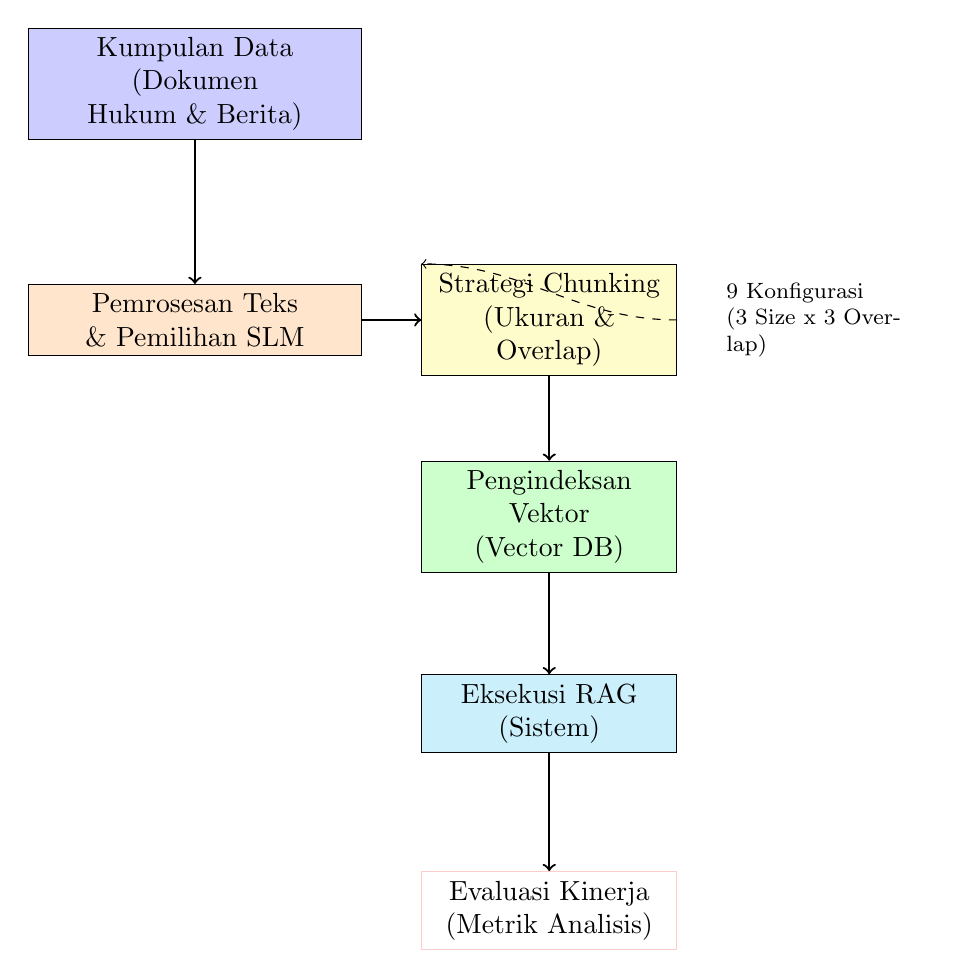
\begin{tikzpicture}[node distance=2.5cm, auto]
        % Definisi Node (Kotak-kotak)
        \node (data) [rectangle, draw, fill=blue!20, text width=4cm, align=center] {Kumpulan Data\\(Dokumen Hukum \& Berita)};
        
        \node (proc) [rectangle, draw, fill=orange!20, below of=data, yshift=-0.5cm, text width=4cm, align=center] {Pemrosesan Teks\\\& Pemilihan SLM};
        
        \node (chunk) [rectangle, draw, fill=yellow!20, right of=proc, xshift=2cm, text width=3cm, align=center] {Strategi Chunking\\(Ukuran \& Overlap)};
        
        \node (index) [rectangle, draw, fill=green!20, below of=chunk, text width=3cm, align=center] {Pengindeksan Vektor\\(Vector DB)};
        
        \node (rag) [rectangle, draw, fill=cyan!20, below of=index, text width=3cm, align=center] {Eksekusi RAG\\(Sistem)};
        
        \node (eval) [rectangle, draw, draw=red!20, below of=rag, text width=3cm, align=center] {Evaluasi Kinerja\\(Metrik Analisis)};
        
        % Definisi Panah (Hubungan)
        \draw [->, thick] (data) -- (proc);
        \draw [->, thick] (proc) -- (chunk);
        \draw [->, thick] (chunk) -- (index);
        \draw [->, thick] (index) -- (rag);
        \draw [->, thick] (rag) -- (eval);
        
        % Tambahan: Loop Parameter (Opsional untuk menunjukkan perulangan)
        \node [right of=chunk, xshift=1cm, text width=2.5cm, font=\footnotesize] {9 Konfigurasi\\(3 Size x 3 Overlap)};
        \draw [dashed, ->] (chunk.east) to [out=180,in=0] (chunk.north west);
    \end{tikzpicture}
    \caption{Diagram Alur Penelitian}
    \label{fig:alur_penelitian}
\end{figure}

\subsection{Pengumpulan Data dan Korpus Pengetahuan}
Dalam penelitian ini, digunakan dua sumber data dokumen utama untuk membentuk Korpus Pengetahuan (\textit{Knowledge Base}) bagi sistem \textit{RAG}. Pemilihan dokumen didasrkan pada representatitas teks publik di Indonesia yang sering diakses masyarakat, yaitu dokumen hukum/pemerintah dan berita.
\subsection{Pemilihan Model}
Untuk mengevaluasi performa dari SLM pada \textit{hardware} dengan sumber daya terbatas namun masih tetap mendapatkan nilai akurasi yang tinggi untuk Bahasa Indonesia, peneliti memilih 3 model dengan ukuran parameter sekitar 3 miliar (3B) yang telah dioptimalkan untuk inferensi khususnya untuk bahasa Indonesia. Model yang dipilih menyeimbangkan kemampuan multibahasa global dengan optimisasi performa bahasa khususnya bahasa-bahasa di Asia Tenggara khususnya Indonesia. Berikut 3 model yang dipilih:
\begin{itemize}
    \item \textbf{Qwen2.5-3B-Instruct:} Model ini digunakan sebagai \textit{baseline} global multilingual model. Model ini merupakan bagian dari \textit{Qwen2.5} series yang dikembangkan oleh Alibaba. Model ini telah mengalami peningkatan yang signifikan pada tahapan \textit{pre-training} dan \textit{post-training} untuk mendukung lebih dari 29 bahasa, termasuk bahasa Indonesia. Menjadikannya model SLM yang tepat sebagai referensi performa global.
    \item \textbf{Sailor2-3B-Chat:} Dipilih sebagai representasi dari model yang telah dioptimalkan khususnya untuk bahasa-bahasa di daerah Asia Tenggara. Model ini secara eksplisit mendukung bahasa Inggris, Chinese, dan bahasa-bahasa di Asia Tenggara termasuk bahasa Indonesia, bahkan bahasa Jawa dan Sunda. Hal ini sejalan dengan temuan pada penelitian sebelumnya yang menunjukkan bahwa model yang dioptimalkan untuk bahasa khusus memiliki performa yang lebih baik dibandingkan model multibahasa global \citep{cahyawijaya-etal-2021-indonlg}
    \item \textbf{SEA-LION-v1-3B:} Model ini merupakan bagian dari seri \textit{SEA-LION} yang dirancang untuk mendukung 11 bahasa di Asia Tenggara, khususnya Indonesia, Vietnam, dan Thailand. Peneliti memilih model dengan 3 miliar parameter (3B) untuk menjaga konsistensi dengan model lain yang digunakan dalam eksperimen.
\end{itemize}
Dikarenakan penelitian ini memiliki batasan pada sumber daya yang digunakan, ketiga model diatas menggunakan versi \textit{quantized (4-bit atau 8-bit)} untuk memastikan supaya dapat dioperasikan dengan batasan memori yang terbatas (RAM 16GB dan Onboard GPU), sehingga memungkinkan penggunaan model SLM secara lokal tanpa perlu akses ke \textit{cloud computing} berskala enterprise.
Eksperimen akan dilakukan dengan skema berikut:
\begin{itemize}
    \item \textbf{Sistem RAG Lokal:} Membangun pipeline menggunakan framework LangChain atau LlamaIndex.
    \item \textbf{Konfigurasi Model:} Model akan dijalankan dalam format GGUF (4-bit quantization) agar dapat dimuat sepenuhnya ke dalam RAM 16GB dan berjalan lancar di Onboard GPU (Intel Iris) menggunakan inferensi engine seperti llama.cpp atau Ollama.
\end{itemize}

\subsection{Strategi Pemotongan Teks (\textit{Chunking}) dan \textit{Overlap}}
Untuk mengatasi batasan panjang konteks (\textit{context window}) pada model SLM dan mengoptimalkan akurasi proses \textit{retrieval}, dokumen dipotong-potong menjadi beberapa bagian teks yang lebih kecil (\textit{chunk}).
\begin{itemize}
  \item Teknik Pemotongan (\textit{Chunking Strategy}): Metode pemotongan yang idgunakan adalah \textbf{\textit{Fixed-Size Chunking}} dengan pendekatan \textit{Recursive Character Splitter}. Metode ini membagi teks berdasarkan jumlah karakter dengan menghormati batasan semantik alami (seperti paragraf dan kalimat) terlebih dahulu \citep{langchain2025splitter}. Implementasi dalam penelitian ini menggunakan prioritas pemisah ganda pada baris baru (\texttt{\textbackslash n\textbackslash n}), baris baru (\texttt{\textbackslash n}), dan akhirnya spasi.
  \item Variabel Ukuran \textit{Chunk}: Penelitian ini menguji tiga konfigurasi ukuran \textit{chunk} untuk menemukan titik keseimbanganantara konteks dan presisi:
    \begin{itemize}
        \item \textbf{128 token}: Ukuran kecil yang diharapkan memberikan presisi tinggi dalam \textit{retrieval} namun memiliki risiko kehilangan konteks antar potongan.
        \item \textbf{256 token}: Ukuran menengah yang sering digunakan sebagai default dalam praktik \textit{RAG}.
        \item \textbf{512 token}: Ukuran besar yang diharapkan memberikan konteks yang lebih luas namun mungkin mengurangi presisi karena memasukkan informasi-informasi yang kurang relevan (\textit{noise}) ke dalam jawaban.
    \end{itemize}
\end{itemize}

\subsection{Variabel \textit{Overlap} (Tumpang Tindih)}
Untuk memitigasi risiko pemutusan informasi di antar batas chunk, diterapkan mekanisme overlap (perulangan teks). Tiga persentase overlap yang diuji adalah: 

\begin{itemize}
     \item 0\%: Sebagai kontrol ablasi untuk mengukur dampak pemisahan total tanpa tumpang tindih.
     \item 10\%: Persentase tumpang tindih yang direkomendasikan dalam praktik terbaik untuk menjaga koherensi konteks \citep{weaviate2024chunking}.
     \item 20\%: Tumpang tindih yang lebih besar untuk memastikan tidak ada informasi krusial yang terlewat di batas antar chunk.
\end{itemize}

Dengan kombinasi 3 ukuran chunk dan 3 persentase overlap, terdapat total 9 konfigurasi pemrosesan dokumen yang akan diuji pada setiap model. 

\subsection{Desain Sistem \textit{Retrieval-Augmented Generation (RAG)}} 

Sistem RAG yang dibangun dalam penelitian ini mengadopsi arsitektur standar yang terdiri dari tiga komponen utama: \textit{Retriever}, \textit{Knowledge Base}, dan \textit{Generator}. 

\begin{itemize}
  \item Representasi Vektor dan Pengindeksan \textit{(Vector Embedding \& Indexing)} \par
  Setiap chunk dokumen diubah menjadi representasi numerik (\textit{embeddings}) menggunakan model \textit{embedding multilingual} yang tetap untuk seluruh eksperimen. Pilihan embedding model ini bertujuan untuk memastikan bahwa perbedaan kinerja yang teramati disebabkan oleh strategi chunking atau model SLM, bukan oleh perbedaan metode retrieval. Vektor hasil \textit{embedding} kemudian disimpan dalam indeks vektor menggunakan \textit{FAISS (Facebook AI Similarity Search)} untuk memungkinkan pencarian cepat dan efisien. 
  \item Mekanisme Retrieval \par
  Saat menerima pertanyaan dari pengguna, sistem akan mengubah pertanyaan menjadi vektor menggunakan embedding model yang sama. Kemudian, sistem melakukan pencarian kemiripan (\textit{nearest neighbor search}) di dalam indeks vektor untuk mengambil top-k dokumen yang paling relevan. Dalam penelitian ini, nilai k=5 ditetapkan sebagai jumlah chunk yang akan diberikan kepada model \textit{SLM} sebagai konteks tambahan. 
  \item Generasi Jawaban (\textit{Answer Generation}) \par
  \textit{Chunk} yang berhasil diambil dan pertanyaan pengguna kemudian diformat menjadi satu prompt (\textit{prompt engineering}) yang dimasukkan ke dalam model \textit{SLM}. Model \textit{SLM} bertugas untuk membaca konteks yang diberikan dan menyusun jawaban yang relevan dan koheren berdasarkan informasi tersebut. 
\end{itemize}

\begin{figure}[H]
    \centering
    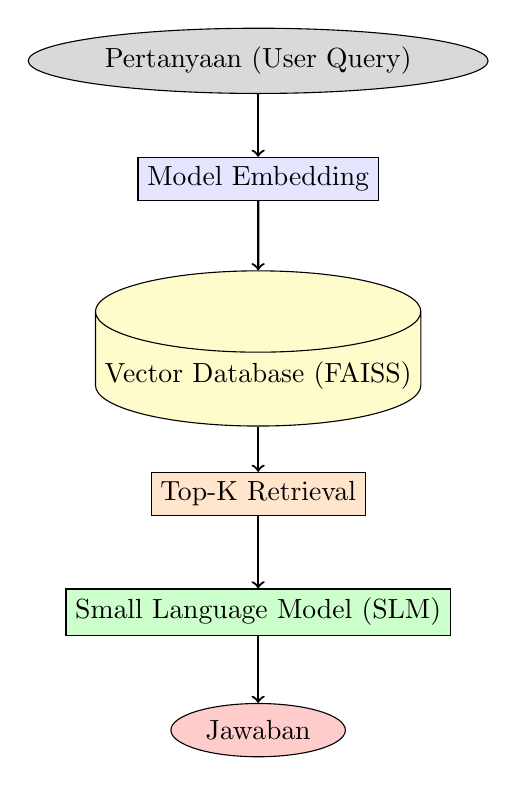
\begin{tikzpicture}[node distance=1.5cm, auto]

        \node (user) [draw, ellipse, fill=gray!30] {Pertanyaan (User Query)};
        
        \node (embed) [draw, rectangle, fill=blue!10, below of=user] {Model Embedding};
        
        \node (db) [draw, cylinder, shape border rotate=90, yshift=-1cm, aspect=0.25, fill=yellow!20, below of=embed] {Vector Database (FAISS)};
        
        \node (retr) [draw, rectangle, fill=orange!20, below of=db] {Top-K Retrieval};
        
        \node (slm) [draw, rectangle, fill=green!20, below of=retr] {Small Language Model (SLM)};
        
        \node (ans) [draw, ellipse, fill=red!20, below of=slm] {Jawaban};
        
        % Panah
        \draw [->, thick] (user) -- (embed);
        \draw [->, thick] (embed) -- (db);
        \draw [->, thick] (db) -- (retr);
        \draw [->, thick] (retr) -- (slm);
        \draw [->, thick] (slm) -- (ans);
    \end{tikzpicture}
    \caption{Arsitektur Sistem RAG}
    \label{fig:rag_vertical_fixed}
\end{figure}

\subsection{Data Pertanyaan untuk Evaluasi}

Untuk mengevaluasi kinerja sistem RAG dan dampak konfigurasi chunking penulis menggunakan 50 pertanyaan sintetis. Pertanyaan yang digunakan dibuat khusus dari korpus dokumen sendiri (UU ITE dan Korpus Berita). Pertanyaan dibuat menggunakan bantuan model bahasa besar lain yang tidak termasuk dalam evaluasi. Langkah ini penting untuk memastikan bahwa setiap pertanyaan memiliki jawaban yang eksplisit terdapat di dalam dokumen. Hal ini memungkinkan pengukuran metrik akurasi (seperti \textit{Recall} atau \textit{F1 Score}) merefleksikan kualitas strategi retrieval dan chunking, bukan sekadar ketiadaan data dalam korpus. 

\subsection{Metrik Evaluasi}

Penelitian ini menggunakan kerangka evaluasi multidimensi untuk mengukur aspek akurasi retrieval, kualitas jawaban generasi, dan efisiensi sistem. 

\begin{itemize}
  \item Metrik Tingkat Retrieval (\textit{Retrieval Metrics}) \par
    Metrik ini mengukur seberapa baik sistem dalam menemukan chunk yang relevan. 
    \begin{itemize}
        \item Recall@k: Persentase pertanyaan di mana setidaknya satu chunk yang relevan (dengan overlap token >50\% terhadap ground-truth passage) muncul dalam top-k hasil pencarian.
        \item Precision@k: Persentase chunk yang relevan di antara top-k hasil pencarian.
    \end{itemize}
     
  \item Metrik End-to-End RAG (Generasi)\par
    Untuk mengukur kualitas jawaban yang dihasilkan oleh model SLM berdasarkan konteks yang diambil, digunakan kerangka evaluasi \textit{RAGAS (Retrieval Augmented Generation Assessment)} \citep{es2025ragasautomatedevaluationretrieval}. 
    \begin{itemize}
        \item \textit{Faithfulness} (Kejujuran): Mengukur sejauh mana jawaban yang dihasilkan didukung oleh fakta yang terdapat dalam konteks yang diambil (\textit{groundedness}). Nilai \textit{faithfulness} yang tinggi menandakan rendahnya halusinasi.
        \item \textit{Answer Relevancy} (Relevansi Jawaban): Mengukur sejauh mana jawaban dihasilkan langsung menjawab pertanyaan pengguna tanpa menyimpang keluar topik.
        \item \textit{Context Precision}: Mengukur rasio sinyal-terhadap-noise pada konteks yang diambil, yaitu berapa banyak chunk yang diambil yang benar-benar relevan.
        \item \textit{Context Recall}: Mengukur kemampuan sistem untuk menemukan seluruh informasi yang diperlukan dari korpus untuk menjawab pertanyaan tersebut.
    \end{itemize}
     
  \item Metrik Efisiensi (Efficiency Metrics)\par
    Mengingat batasan perangkat keras terbatas yang digunakan (laptop standar), efisiensi sistem menjadi faktor penting. 
    \begin{itemize}
     \item Average Latency (Latensi Rata-rata): Waktu yang dibutuhkan sistem dari menerima input pertanyaan hingga menghasilkan jawaban akhir (dalam detik).
     \item Peak Memory Usage: Penggunaan memori maksimum (RAM/VRAM) selama proses inferensi untuk setiap konfigurasi.
    \end{itemize}
\end{itemize}

\subsection{Prosedur Eksperimen}
Prosedur eksperimen dilakukan secara sistematis untuk memastikan reproduktibilitas hasil. 
\begin{itemize}
    \item Persiapan dan Pemotongan Dokumen: Dokumen dari korpus hukum dan berita dipotong menggunakan skrip Python yang menerapkan \textit{Recursive Character Splitter}. Sembilan kombinasi parameter (\textit{chunk\_size}, \textit{overlap}) yaitu (128, 256, 512) token dan (0\%, 10\%, 20\%) diterapkan untuk menghasilkan set data potongan yang terpisah. 
    \item Pengindeksan Vektor (\textit{Vector Indexing}): Setiap set potongan dikonversi menjadi vektor menggunakan model embedding dan diindeksasikan menggunakan FAISS. Indeks ini disimpan untuk keperluan retrieval secara cepat. 
    \item Pelaksanaan Inferensi: Untuk setiap kombinasi parameter dan setiap model SLM, sistem dijalankan untuk memproses seluruh pertanyaan uji. Sistem mencatat log waktu (latensi) dan penggunaan memori untuk setiap eksekusi. 
    \item Koleksi Hasil dan Perhitungan Metrik: Hasil jawaban dan konteks yang diambil disimpan. Selanjutnya, metrik evaluasi (\textit{Recall}, \textit{F1}, \textit{Faithfulness}, dll.) dihitung. Untuk metrik \textit{RAGAS}, digunakan model \textit{LLM} lain yang lebih besar sebagai "judge" otomatis untuk menilai kualitas jawaban tanpa bias terhadap model \textit{SLM} yang sedang diuji. 
\end{itemize}



% --- REFERENCES ---
\setlength{\parindent}{0cm} % Bibliography usually hanging indent handled by package, but reset parindent here just in case.
\bibliographystyle{apalike} % Or any style matching "Author-Year" [34]
\bibliography{referensi}    % Expects a referensi.bib file
% \addcontentsline{toc}{chapter}{DAFTAR PUSTAKA}
\bibsection

% --- APPENDIX ---
\chapter*{LAMPIRAN}
\addcontentsline{toc}{chapter}{LAMPIRAN}
% [9] Lampiran: Surat izin, kuesioner, data, dll.

\end{document}

%%% Local Variables:
%%% mode: LaTeX
%%% TeX-master: t
%%% End: